\chapter{Implémentation}
\begin{spacing}{1.2}
\minitoc
\thispagestyle{MyStyle}
\end{spacing}
\newpage

\section{INTRODUCTION}
Ce chapitre constitue le cœur de notre projet, où chaque ligne de code représente une étape vers la réalisation de notre vision.
Dans cette section, nous plongerons dans les détails techniques de l'implémentation de notre solution. Nous explorerons les choix d'architecture, les langages de programmation utilisés, ainsi que les bibliothèques et les outils spécifiques nécessaires pour atteindre nos objectifs. Nous décrirons également les différentes étapes de développement, depuis la configuration initiale jusqu'aux tests et à l'optimisation.
À travers cette plongée dans le code, nous chercherons à illustrer non seulement la manière dont notre solution fonctionne, mais aussi les défis rencontrés et les solutions apportées.  
 
 \section{Choix de technologies utilisé}
 
 Pour le calibrage de la caméra et l'estimation des performances, un système de vision par ordinateur est essentiel. La vision par ordinateur est un domaine de l'informatique qui se concentre sur l'acquisition, le traitement et l'analyse des images numériques afin de comprendre et d'interpréter le contenu visuel du monde réel. Elle vise à donner aux ordinateurs la capacité de "voir" et de comprendre des images de la même manière que le font les êtres humains.
 Nous avons utlisé plusieurs langages de programmation et bibliothèques qui sont entre autre : 
 
  \begin{itemize}[label={\Huge$\star$}]
  
  \item \textbf{Langages de programmation :}
  
  		\begin{itemize}
  			\item \textbf{Python :} est largement utilisé dans le domaine de la vision par ordinateur et du traitement d'images en raison de sa simplicité, de sa flexibilité et de sa richesse en bibliothèques
  		\end{itemize}
  		
  \item \textbf{Bibliothèques Python}
  
  		\begin{itemize}
  			\item \textbf{NumPy:} est une bibliothèque Python pour le calcul numérique. Elle fournit des structures de données efficaces pour la manipulation de tableaux multidimensionnels, ce qui est essentiel pour le traitement d'images et l'analyse des données.
  			
  			\item \textbf{OpenCV (Open Source Computer Vision Library) :} est une bibliothèque de vision par ordinateur open source largement utilisée pour le traitement et l'analyse d'images et de vidéos. Développée initialement par Intel, OpenCV est maintenant maintenue par une large communauté de contributeurs. La bibliothèque est conçue pour fournir une infrastructure commune pour les applications de vision par ordinateur et pour faciliter l'intégration de la perception des machines dans divers produits commerciaux.
  			
  			\item \textbf{Matplotlib:} est une bibliothèque de visualisation en 2D pour Python. Elle est souvent utilisée pour créer des graphiques et des visualisations à partir des données extraites des vidéos, ce qui est utile pour l'analyse des performances des sauts en longueur.
  			
  			\item\textbf{Glob:}  est utilisé pour rechercher des chemins de fichiers ou de répertoires correspondant à un modèle de recherche spécifié en utilisant des motifs de correspondance de style Unix.
  			
  			\item \textbf{Pickle:} est un module Python qui permet de sérialiser et de désérialiser des objets Python. La sérialisation consiste à convertir un objet Python en une représentation de données pouvant être écrite sur le disque ou transmise sur un réseau, tandis que la désérialisation consiste à reconstituer l'objet à partir de cette représentation de données.
  		\end{itemize}
  
 \item \textbf{IDE utilisé}	
  			
  			Nous avons installé \textbf{Anaconda}  pour pouvoir utlisé \textbf{Jupyter Notebook}. Anaconda est une plateforme open-source facilitant la gestion des packages, des environnements virtuels et des ressources pour le développement et l'analyse de données.
  			Jupyter Notebook quand à lui est une application web open-source qui permet de créer et de partager des documents interactifs contenant du code, des visualisations et du texte explicatif.
\end{itemize}
 
 
 \newpage
\section{Code de calibrage de la caméra}
 Notre code de calibrage sera éffectué en  étapes principales et dans plusieurs fichiers différents.
 
  \subsection{Première étape : Capture d'image}
 		
 	Cette partie du code nous permet d'ouvrir une interface nommée \textbf{"Img"} de notre caméra en temps réèl et de capturer des images en nombre voulue en appuyant sur la touche \textbf{"S"}. Cette interface peut être refermer en appuyant sur la touche \textbf{"echap"}. Les images capturé sont automatiquement enregistré dans le repertoire \textbf{"image"} et une notification du type \textbf{"image enregistrer"} est présenté comme résultat.
 	
 	\begin{figure}[H]%
 		\center%
 		\setlength{\fboxsep}{5pt}%
 		\setlength{\fboxrule}{0.5pt}%
 		\fbox{
 			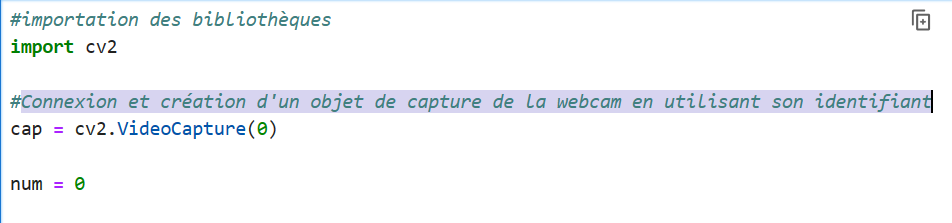
\includegraphics[scale=0.6]{images/captureimage1}
 		}
 		\caption[Code de capture d'image (partie 1)]{Connexion et création d'un objet de capture de la webcam en utilisant son identifiant. Source : Photos prise sur notre machine}%
 		\label{fig:Code de capture d'image(partie 1)}
 	\end{figure}
 	
 	
 	\begin{figure}[H]%
 		\center%
 		\setlength{\fboxsep}{5pt}%
 		\setlength{\fboxrule}{0.5pt}%
 		\fbox{
 			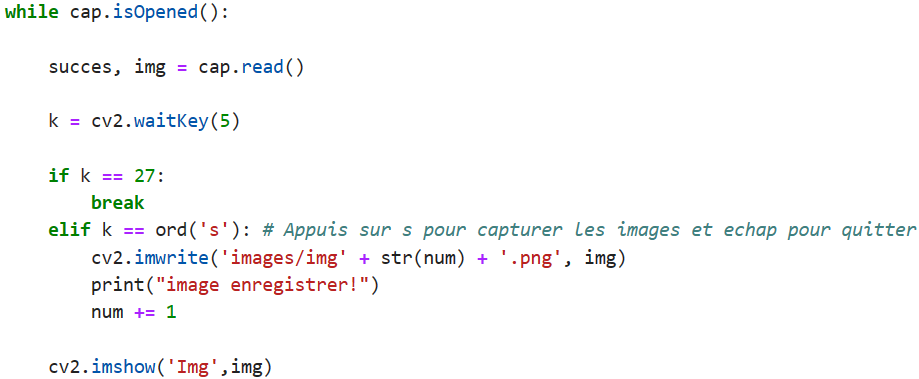
\includegraphics[scale=0.6]{images/captureimage2}
 		}
 		\caption[Code de capture d'image (partie 2)]{Boucle permetant d'ouvrir l'interface de la caméra et de prendre des images. Source : Photos prise sur notre machine}%
 		\label{fig:Code de capture d'image(partie 2)}
 	\end{figure}
 	
 	\begin{figure}[H]%
 		\center%
 		\setlength{\fboxsep}{5pt}%
 		\setlength{\fboxrule}{0.5pt}%
 		\fbox{
 			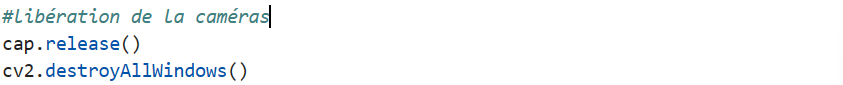
\includegraphics[scale=0.6]{images/captureimage3}
 		}
 		\caption[Code de capture d'image (partie 3)]{ Libération de la caéra. Source : Photos prise sur notre machine}%
 		\label{fig:Code de capture d'image(partie 3)}
 	\end{figure}
 	
 	\begin{figure}[H]%
 		\center%
 		\setlength{\fboxsep}{5pt}%
 		\setlength{\fboxrule}{0.5pt}%
 		\fbox{
 			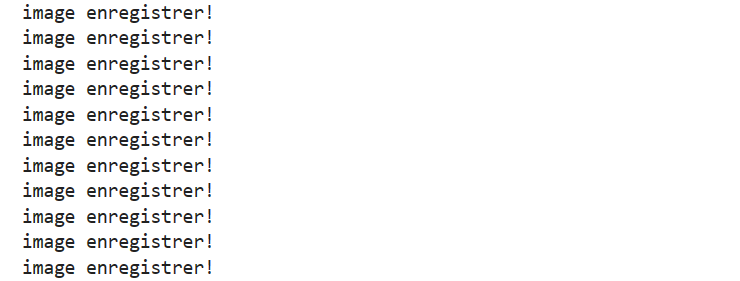
\includegraphics[scale=0.6]{images/captureimage4}
 		}
 		\caption[ Résultat du code de capture d'image ]{ Résultat du code de capture d'image. Source : Photos prise sur notre machine}%
 		\label{fig:Résultat du code de capture d'image}
 	\end{figure}
 	
 	\begin{figure}[H]%
 		\center%
 		\setlength{\fboxsep}{5pt}%
 		\setlength{\fboxrule}{0.5pt}%
 		\fbox{
 			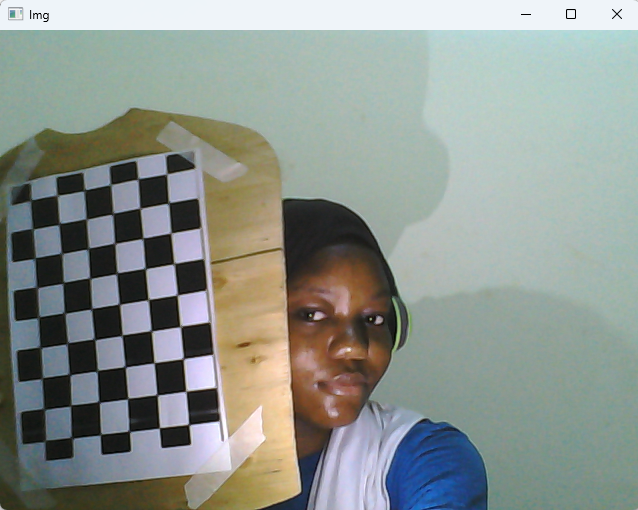
\includegraphics[scale=0.6]{images/interface}
 		}
 		\caption[Interface de la caméra ]{ Interface en temp réèl de la caméra. Source : Photos prise sur notre machine}%
 		\label{fig:Interface de la caméra}
 	\end{figure}
 	
 	\subsection{ Deuxième partie : Définition des coordonnées du monde réèl}
  	
 	Nous avons défini les coordonnées du monde réèl à l'aide du motif de damier de taille \textbf{(9,6)}. La taille se compte par l'intersection des carrés du damier horizontalement et verticalement.
 	
 	 \begin{figure}[h]
 	 	\centering
 	 	\fbox{
 	 		\begin{minipage}{0.4\textwidth}
 	 			\centering
 	 			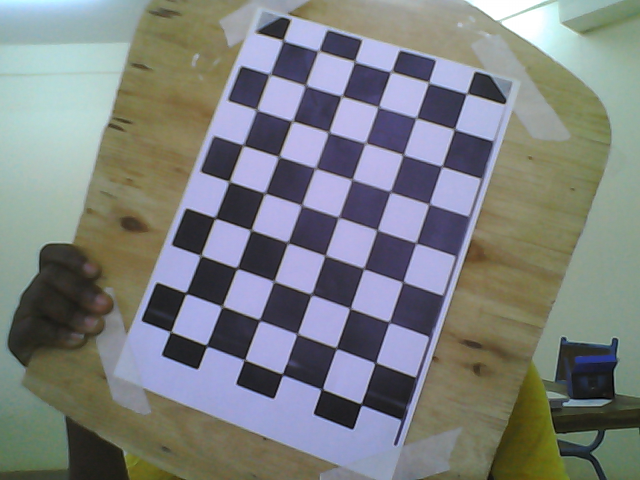
\includegraphics[width=\linewidth]{images/img1}
 	 		\end{minipage}\hfill
 	 		\begin{minipage}{0.4\textwidth}
 	 			\centering
 	 			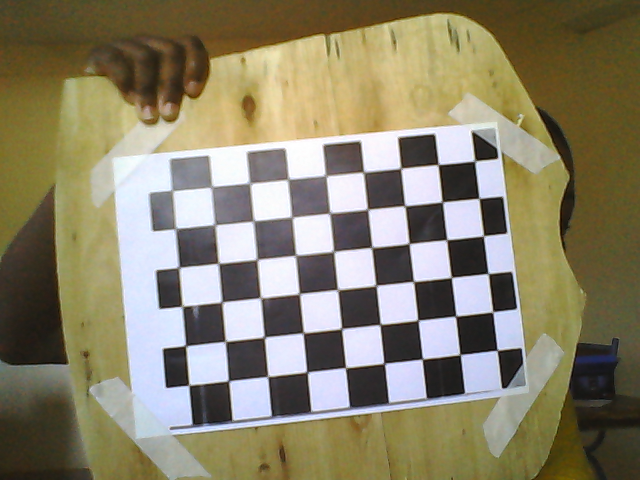
\includegraphics[width=\linewidth]{images/img2}
 	 		\end{minipage}\hfill 
 	 	}
 	 	\caption[Image du damier]{Image du damier prise par notre caméra pour le calibrage. Source : Photos prise sur notre machine}
 	 	\label{fig:Image du damier}
 	 \end{figure}
 	 
 	 \begin{figure}[H]%
 	 	\center%
 	 	\setlength{\fboxsep}{5pt}%
 	 	\setlength{\fboxrule}{0.5pt}%
 	 	\fbox{
 	 		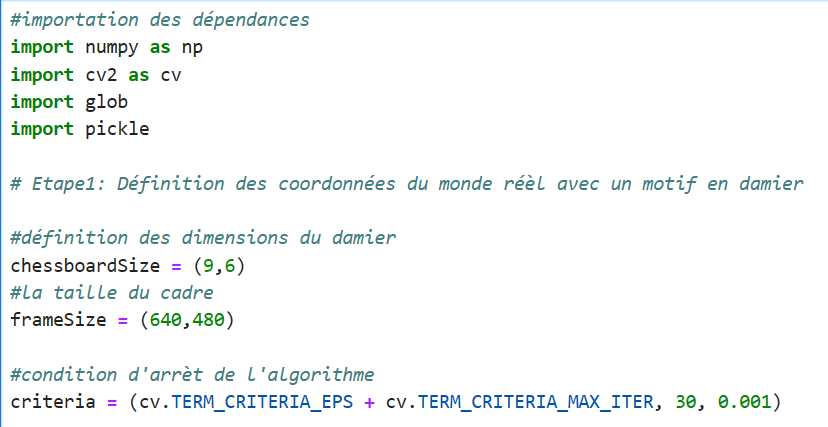
\includegraphics[scale=0.6]{images/3d1}
 	 	}
 	 	\caption[Définition des coordonnées du monde réèl]{Définition des coordonnées du monde réèl avec un motif en damier. Source : Photos prise sur notre machine}
 	 	\label{fig:Définition des coordonnées du monde réèl}
 	 	 \end{figure}
 	 	 \begin{figure}[H]%
 	 		\center%
 	 		\setlength{\fboxsep}{5pt}%
 	 		\setlength{\fboxrule}{0.5pt}%
 	 		\fbox{
 	 			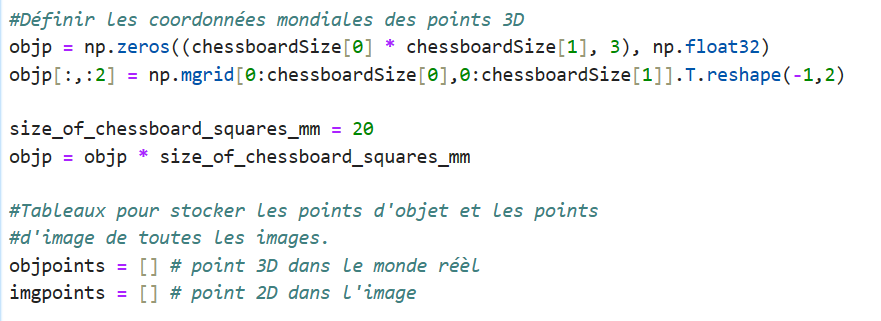
\includegraphics[scale=0.6]{images/3d2}
 	 		}
 	 		\caption[Définition des coordonnées du monde réèl(suite)]{Définition des coordonnées du monde réèl avec un motif en damier(suite). Source : Photos prise sur notre machine}
 	 		\label{fig:Définition des coordonnées du monde réèl(suite)}
 	 		 \end{figure}
 	 
 	
 	\subsection{Troisième partie : Définition des points d'objets et des points images}
 	 
 	Pour ce faire, nous avons utilisé trois fonctions de \textbf{Opencv} à savoir \textbf{cv.findChessboardCorners()}, \textbf{cv.cornerSubPix} , \textbf{cv.drawChessboardCorners()} pour trouver, afiner et déssiner les coins du damier. Nous allons charger les images prise grâce au code de la première partie. 
 	
 	 \begin{figure}[H]%
 		\center%
 		\setlength{\fboxsep}{5pt}%
 		\setlength{\fboxrule}{0.5pt}%
 		\fbox{
 			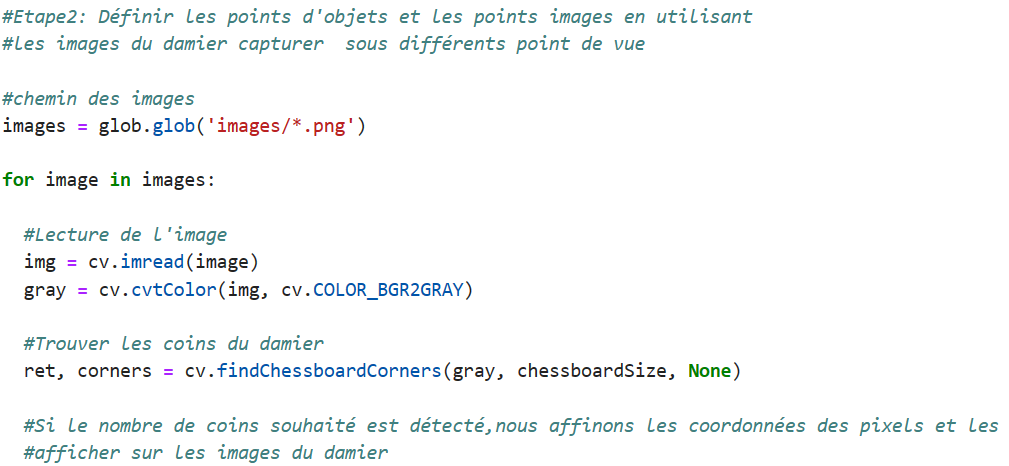
\includegraphics[scale=0.6]{images/point1}
 		}
 		\caption[Définition des points d'objets et points images]{Définition des points d'objets et des points images. Source : Photos prise sur notre machine}
 		\label{fig:Définition des points d'objets et des points images}
 	\end{figure}
 	
 	\begin{figure}[H]%
 		\center%
 		\setlength{\fboxsep}{5pt}%
 		\setlength{\fboxrule}{0.5pt}%
 		\fbox{
 			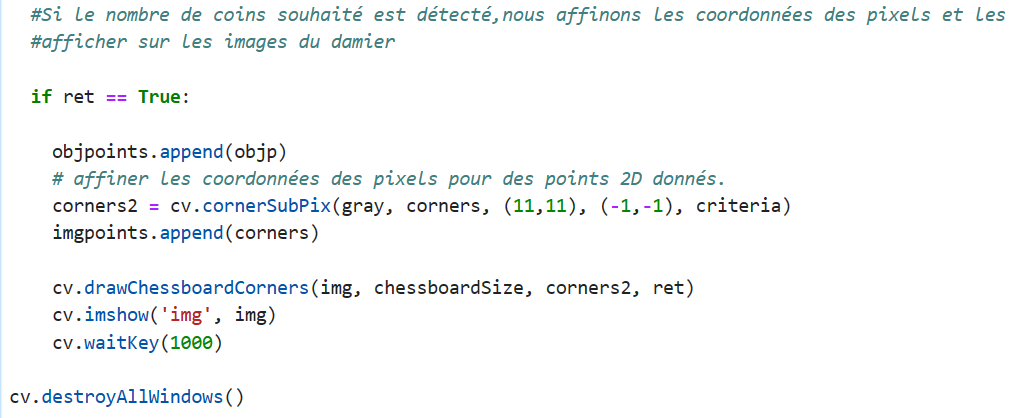
\includegraphics[scale=0.6]{images/point2}
 		}
 		\caption[Définition des points d'objets et points images(suite)]{Définition des points d'objets et des points images(suite). Source : Photos prise sur notre machine}
 		\label{fig:Définition des points d'objets et des points images(suite)}
 	\end{figure}
 	
  
 \subsection{Quatrième partie : Calibrage}
 
 Une fois les code des trois étapes au dessus ont donné les résultats attendu nous avons utilisé la fonction \textbf{cv.calibratecamera}, qui retourne la matrice de la caméra contenant la focale fx et fy, et les centres optiques cx et cy, les paramètres de distortion, les vecteurs de rotation et de translation.
 
 \begin{figure}[H]%
 	\center%
 	\setlength{\fboxsep}{5pt}%
 	\setlength{\fboxrule}{0.5pt}%
 	\fbox{
 		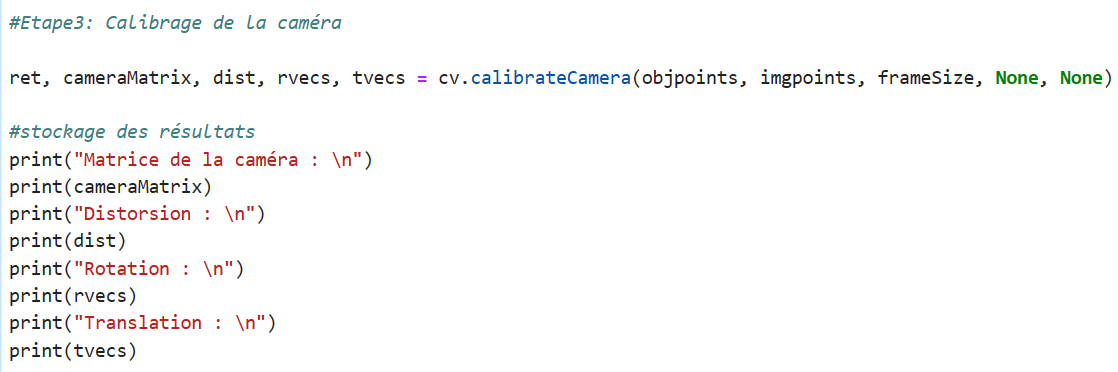
\includegraphics[scale=0.5]{images/calibrage}
 	}
 	\caption[Fonction de calibrage]{Fonction de calibrage. Source : Photos prise sur notre machine}
 	\label{fig:Fonction de calibrage}
 \end{figure}

Quand on exécute le code une fenêtre \textbf{Img} s'ouvre en montrant le processus du calibrage sur les images prise du damier. 

\begin{figure}[H]%
	\center%
	\setlength{\fboxsep}{5pt}%
	\setlength{\fboxrule}{0.5pt}%
	\fbox{
		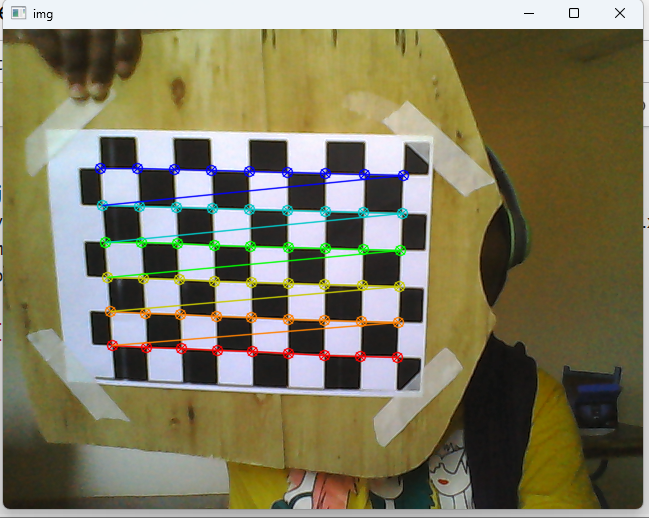
\includegraphics[scale=0.6]{images/calibrage2}
	}
	\caption[Processus de calibrage]{Processus de calibrage. Source : Photos prise sur notre machine}
	\label{fig:Processus de calibrage}
\end{figure}

\vspace{1 cm}
Notre calibrage donne les résultats suivant: 

\begin{figure}[H]%
	\center%
	\setlength{\fboxsep}{5pt}%
	\setlength{\fboxrule}{0.5pt}%
	\fbox{
		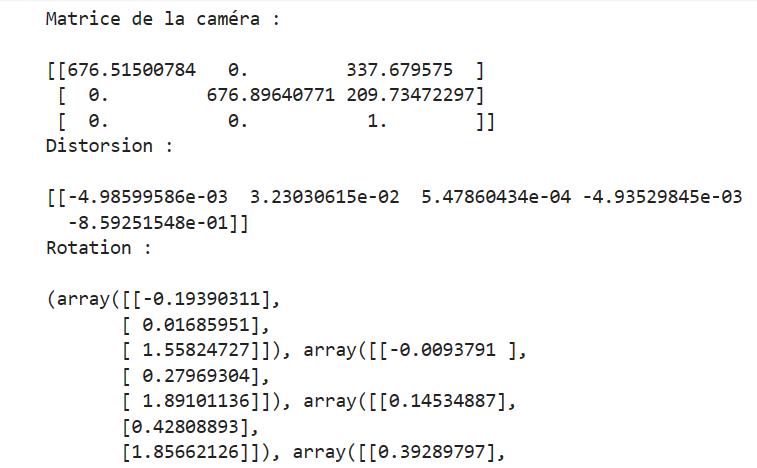
\includegraphics[scale=0.6]{images/resultat1}
	}
	\caption[Résultat du calibrage]{Résultat du calibrage. Source : Photos prise sur notre machine}
	\label{fig:Résultat du calibrage}
\end{figure}

\begin{figure}[H]%
	\center%
	\setlength{\fboxsep}{5pt}%
	\setlength{\fboxrule}{0.5pt}%
	\fbox{
		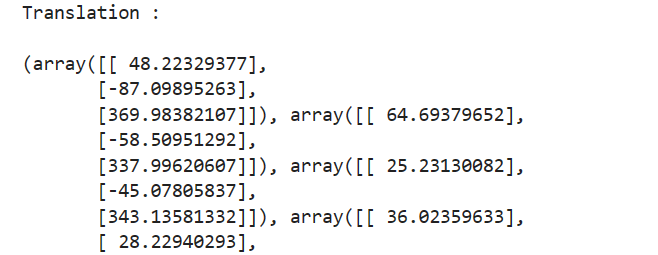
\includegraphics[scale=0.6]{images/resultat2}
	}
	\caption[Résultat du calibrage(suite)]{Résultat du calibrage(suite). Source : Photos prise sur notre machine}
	\label{fig:Résultat du calibrage(suite)}
\end{figure}

\subsection{Cinquième partie : Correction de la distorsion}

On prend une image et on essaye de rectifier les distortions en utilisant les résultats du calibrage.

\begin{figure}[H]%
	\center%
	\setlength{\fboxsep}{5pt}%
	\setlength{\fboxrule}{0.5pt}%
	\fbox{
		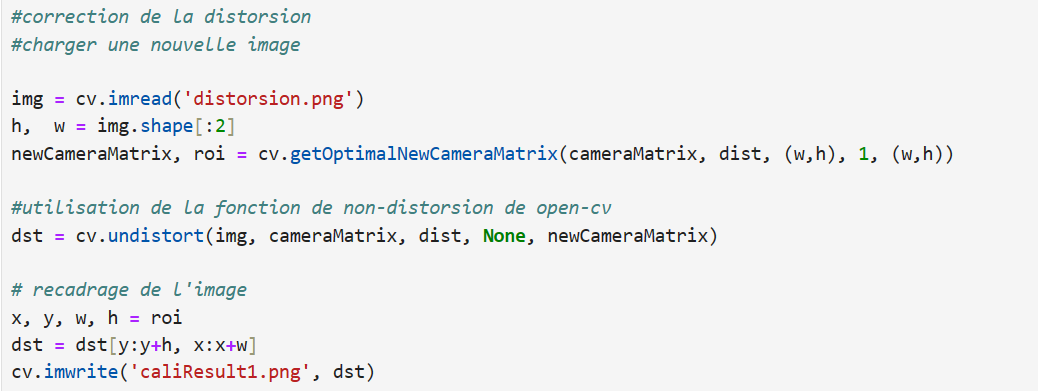
\includegraphics[scale=0.6]{images/distorsion1}
	}
	\caption[Correction de la distorsion sans remapping]{Correction de la distorsion sans remapping. Source : Photos prise sur notre machine}
	\label{fig:Correction de la distorsion sans remapping}
\end{figure}

\begin{figure}[H]%
	\center%
	\setlength{\fboxsep}{5pt}%
	\setlength{\fboxrule}{0.5pt}%
	\fbox{
		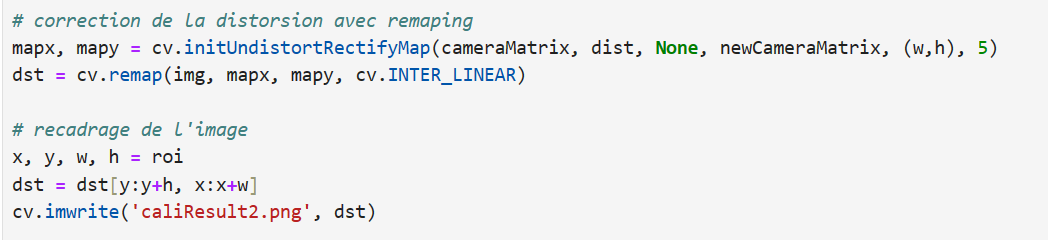
\includegraphics[scale=0.6]{images/distorsion2}
	}
	\caption[Correction de la distorsion avec remapping]{Correction de la distorsion avec remapping. Source : Photos prise sur notre machine}
	\label{fig:Correction de la distorsion avec remapping}
\end{figure}

Voiçi le résultat de la correction de distorsion en image
\begin{figure}[H]%
	\center%
	\setlength{\fboxsep}{5pt}%
	\setlength{\fboxrule}{0.5pt}%
	\fbox{
		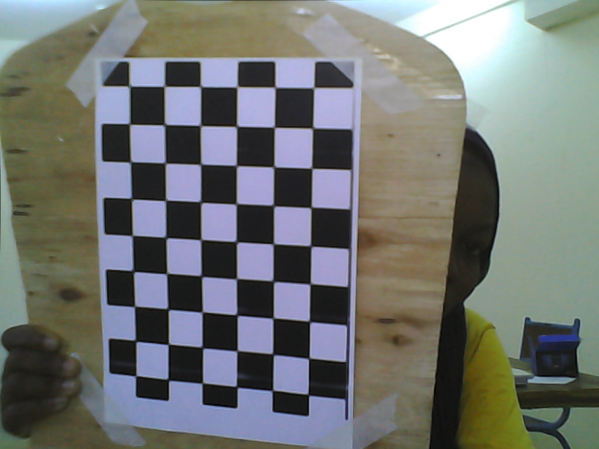
\includegraphics[scale=0.5]{images/resultat4}
	}
	\caption[Résutat de la correction de la distorsion]{Résutat de la correction de la distorsion. Source : Photos prise sur notre machine}
	\label{fig:Résutat de la correction de la distorsion}
\end{figure}

\subsection{L'érreur de calibrage}

Cette partie du code nous permet d'évaluer la précision et la qualité du calibrage.

\begin{figure}[H]%
	\center%
	\setlength{\fboxsep}{5pt}%
	\setlength{\fboxrule}{0.5pt}%
	\fbox{
		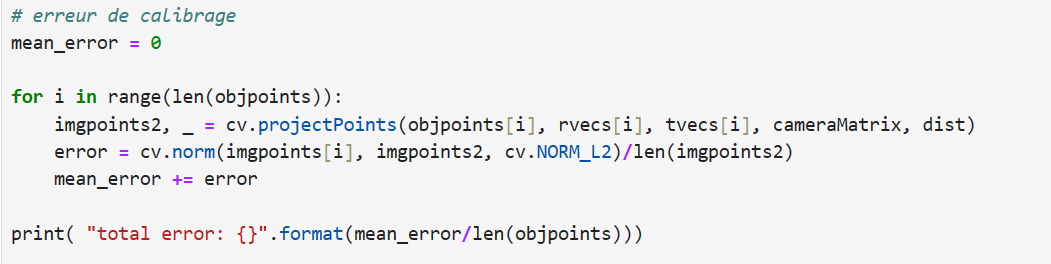
\includegraphics[scale=0.6]{images/erreur}
	}
	\caption[Erreur de calibrage(code)]{Erreur de calibrage(code). Source : Photos prise sur notre machine}
	\label{fig:Erreur de calibrage(code)}
\end{figure}

 
On a une erreur de :


\begin{figure}[H]%
	\center%
	\setlength{\fboxsep}{5pt}%
	\setlength{\fboxrule}{0.5pt}%
	\fbox{
		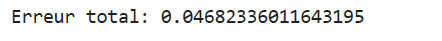
\includegraphics[scale=1]{images/resultat3}
	}
	\caption[ Erreur de calibrage(résultat)]{Erreur de calibrage(résultat). Source : Photos prise sur notre machine}
	\label{fig:Erreur de calibrage(résultat)}
\end{figure}






%\newpage
%\section{Code de calcul de distance sur une image}
 
 %Avec notre caméra déjà calibrée, nous pouvons déterminer la distance entre deux objets en mesurant leurs positions dans l'image et en utilisant les paramètres de calibrage pour convertir ces positions en distances réelles.
 
 
 %\begin{itemize}[label={\Huge$\star$}]
 	%\item \textbf{Détection d'objet}
 	
 	%Pour la détection d'objet nous allons utilisé un modèle pré-entraîné YOLO (You Only Look Once). Pour ce faire nous allons télécharger les fichiers nécessaires pour YOLOv3 \\
 	%(yolov3.weights,yolov3.cfg,coco.names) à partir du référentiel officiel de Darknet\cite{noauthor_yolo_nodate} \cite{noauthor_darknetdatacoconames_nodate,noauthor_darknetcfgyolov3cfg_nodate}, qui est le cadre utilisé pour entraîner YOLO.
 	
%\end{itemize}
 
 %\newpage
 %Pour ce faire nous devons connaitre la taille réelle des objets dans l'image, ce qui peut être difficile à obtenir uniquement à partir de l'image elle-même, à moins d'avoir une référence de taille dans la scène.
 %Une approche courante consiste à utiliser des objets de référence dont les dimensions réelles sont connues. Par exemple, si nous connaissons la largeur réelle d'un des objets dans la scène, nous pouvons utiliser cette information pour convertir les distances calculées en pixels en mètres.
 %Si la taille réelle de l'objet n'est pas connu et que nous ne disposons pas d'autres objets de référence dont les dimensions réelles sont connues, alors nous pouvons utilisé la méthode de détection d'objets et de suivi détecter la ligne d'appel et le bois placé au point d'atterrissage dans l'image.


 
\section{CONCLUSION}
 
 Ce chapitre a exploré en profondeur l'implémentation des codes essentiels au calibrage des caméras et à la mesure de distance, éléments clés pour l'estimation des performances lors des sauts en longueur. Nous avons tout d'abord exploré les langages de programmation utilisés,les bibliothèques et les outils spécifiques nécessaires pour la réalisation du projet.
 
 Ensuite, nous avons détaillé le processus de calibrage, qui inclut la détermination des paramètres intrinsèques et extrinsèques de la caméra, permettant ainsi de corriger les distorsions et d'assurer une correspondance précise entre les coordonnées de l'image et celles du monde réel. Les algorithmes et les techniques utilisés pour ce calibrage, tels que la méthode de Zhang Zhengyou, ont été expliqués et illustrés par des exemples de code.
 
 Enfin, nous avons abordé la mesure de distance à l'aide d'une caméra calibrée. En appliquant des techniques de vision par ordinateur telles que la triangulation stéréoscopique ou l'analyse de la profondeur à partir d'une seule caméra, nous avons démontré comment convertir les informations bidimensionnelles en données tridimensionnelles précises. Les exemples de code fournis ont illustré ces méthodes, montrant comment les données de calibrage sont intégrées pour estimer les distances avec une grande exactitude.
 
  